\documentclass[review]{elsarticle}

\usepackage{lineno,hyperref}

\usepackage{todonotes}
\usepackage{makecell}
\usepackage{graphicx}
\usepackage{adjustbox}
\usepackage{paralist}
\usepackage{amsmath}
\usepackage{booktabs}
\usepackage{tabularx}
\usepackage{cleveref}

\modulolinenumbers[5]
\renewcommand\theadalign{rb}
\newcolumntype{R}[1]{>{\tiny\raggedleft\arraybackslash}b{#1}}

% Comment the following for final version
\setlength{\marginparwidth}{4cm} % expand note margin
%%%%%%%%%%%%%%%%%%%%%%%


\journal{Journal of \LaTeX\ Templates}
\bibliographystyle{elsarticle-num}

\newcommand{\trademark}{{\tiny\textsuperscript\textregistered}}

% Flag that controls the display of comments.
\newif\ifcomments

% Enable/Disable comments.
\commentstrue
% \commentsfalse

\newcommand{\claudio}[1]{%
\ifcomments %
\textbf{\textcolor{red}{\scriptsize Claudio: #1}} %
\else %
 %
\fi%
}%

\newcommand{\gerald}[1]{%
\ifcomments %
\textbf{\textcolor{blue}{\scriptsize Gerald: #1}} %
\else %
 %
\fi%
}%

\newcommand{\sepp}[1]{%
\ifcomments %
\textbf{\textcolor{green}{\scriptsize Sepp: #1}} %
\else %
 %
\fi%
}%

\newcommand{\georg}[1]{%
\ifcomments %
\textbf{\textcolor{yellow}{\scriptsize Georg: #1}} %
\else %
 %
\fi%
}%

\newcommand{\irene}[1]{%
\ifcomments %
\textbf{\textcolor{black}{\scriptsize Irene: #1}} %
\else %
 %
\fi%
}%


\newcommand{\thierry}[1]{%
\ifcomments %
\textbf{\textcolor{green}{\scriptsize Thierry: #1}} %
\else %
 %
\fi%
}%


\begin{document}

\begin{frontmatter}

\title{DEPRECATED. Please follow link in abstract to the correct overleaf project.}

        \author[tug]{G.~Schweiger}
        \author[ant]{C.~Gomes }
        \author[tug]{G.~Engel}
        \author[dwh]{I.~Hafner}
        \author[swe]{J.~Schoeggl}
        \author[kfu]{A. Posch}
        \author[lbnl]{T.~Nouidui \corref{cor1}}

        \address[tug]{Technical University of Graz, Austria}
        \address[ant]{University of Antwerp, Antwerp, Belgium}
        \address[dwh]{dwh GmbH - Simulation Services and Technical Solutions, Vienna, Austria}
        \address[swe]{KTH Royal Institute of Technology, Stockholm, Sweden}
        \address[kfu]{University of Graz, Austria}
        \address[lbnl]{Lawrence Berkeley National Laboratory, Berkeley, USA}


        \cortext[cor1]{Corresponding author. yyy
        000, 000 Berkeley, USA. Tel.: +xxxxxx \textit{E-mail address}: tsnouidui@lbl.gov}

\begin{abstract}

{
\url{https://v2.overleaf.com/5389137161csybdfnnjtmg}
}


\end{abstract}

\begin{keyword}
Co-Simulation \sep Survey \sep Delphi Method
\end{keyword}

\end{frontmatter}

%\linenumbers

\section{Introduction}

Simulation-driven assessments and developments are a key method in various fields in industry and academia such as energy systems, production industry or social sciences. Due to the increasing complexity of systems, market competition, and specialization, it is harder to study the behavior of these systems. 
In order to keep reaping the benefits of simulation, new techniques to efficiently simulate the interactions between subsystems often built by  experts in different disciplines are required. There are two possibilities: (i) the entire system is modelled and simulated in a single tool which is referred to as monolithic simulation; or (ii) established tools for the respective subsystems are coupled in a so-called co-simulation. 

As our knowledge of each subsystem matures, modelling and simulation tools become more specialized, accumulating years of research and practical experience in their respective domains. 
As such, leveraging existing simulation tools, and coupling them in dynamic simulations---co-simulation---, provides a quick and accurate way to realize a holistic simulation by depicting interactions between subsystems while using the most appropriate simulators for each subsystem \cite{VanderAuweraer2013}. 
To assess developments and the importance of co-simulation in the scientific community in recent decades, a keyword analysis was conducted. 
The analysis was performed on \url{www.scopus.com} with the keyword ``co-simulation''. 
\Cref{fig:Publication} shows an almost linear growth of citations from $2000$ to $2017$. As it can be seen in Figure \ref{fig:Subject}, most of the publications are in the field of Engineering (40 \%) followed by Computer Science (25 \%) and Mathematics (11 \%).
Table \ref{tab:projects} gives an overview of research activities in the field of co-simulation in recent years.
%\claudio{I think we should move this paragraph to the previous section, as it motivates the other survey work also done. The current section aims at motivating our work by showing that it complements the existing survey work. Btw it should be clear what each section does and how they fit together.}

\begin{figure}[h!]
\centering
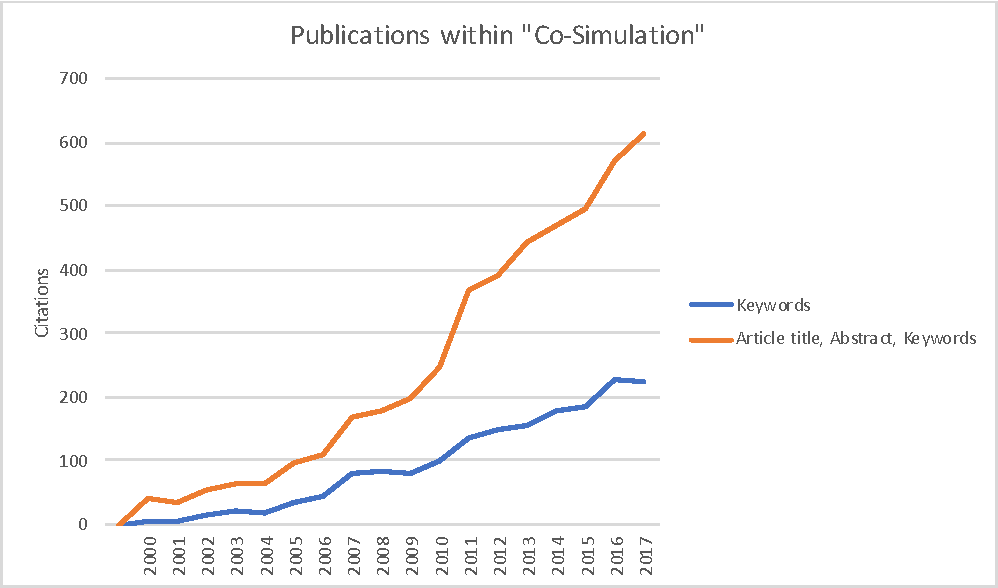
\includegraphics[width=1\textwidth]{Figures/Publications.pdf}
\caption{Publications with the keyword "co-simulation"}
\label{fig:Publication}
\end{figure}

\begin{figure}[h!]
\centering
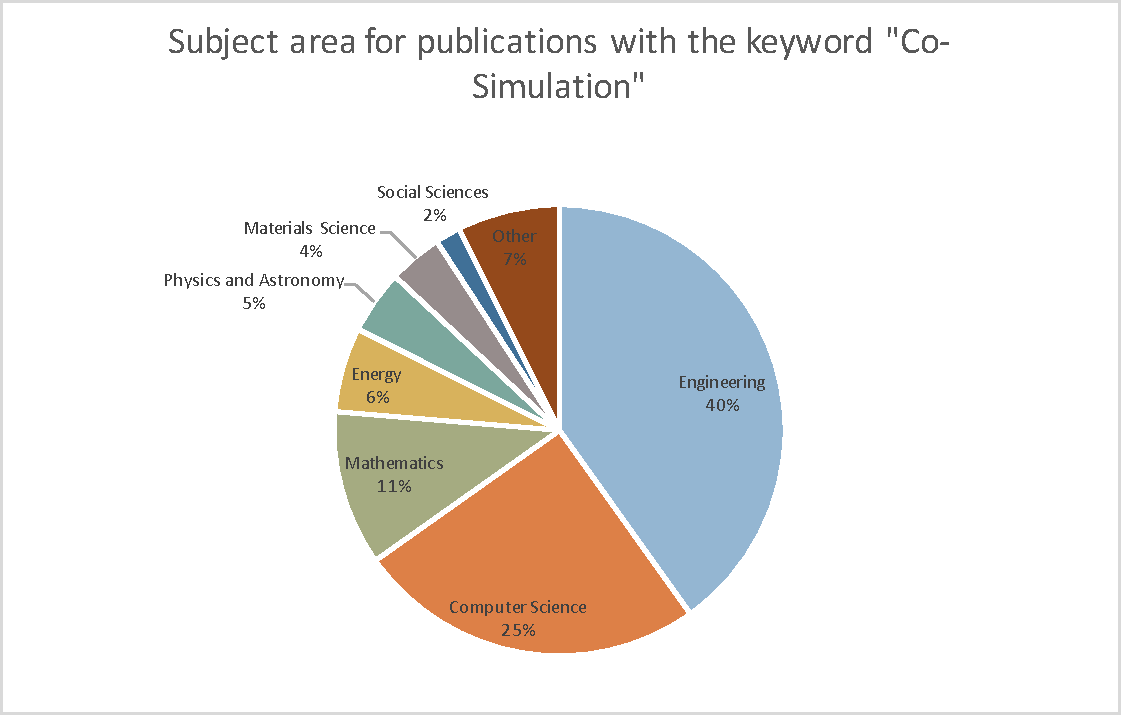
\includegraphics[width=1\textwidth]{Figures/Subject.pdf}
\caption{Subject area for publications with the keyword "co-simulation"}
\label{fig:Subject}
\end{figure}


% Please add the following required packages to your document preamble:
% \usepackage{graphicx}
\begin{table}[]
\caption{Research activities in the field of co-simulation in recent years}
\label{tab:projects}
\resizebox{\textwidth}{!}{%
\begin{tabular}{lll}
\textbf{Project name} & \textbf{Duration} & \textbf{Goals that relate to co-simulation} \\ \hline
COSIBA \cite{cosibas} & 2000 - 2002 & \begin{tabular}[c]{@{}l@{}}The aim was to formulate a co-simulation backplane for coupling electronic design automation tools, \\ that supports co-design using variousspecication formalisms at dierent abstraction levels.\end{tabular} \\
ODETTE \cite{odette} & 2000 - 20003 & \begin{tabular}[c]{@{}l@{}}The aim was to develop and market a complete co-design solution including hardware/software \\ co-simulation and synthesis tools.\end{tabular} \\
MODELISAR \cite{modelisar} & 2008 - 2011 & \begin{tabular}[c]{@{}l@{}}The aim was to improve the design of systems and of embedded software in vehicles. \\ One of the main results was the FMI standard.\end{tabular} \\
DESTECS \cite{destecs} & 2010 - 2012 & \begin{tabular}[c]{@{}l@{}}The aim was to improve the development of fault-tolerant embedded systems, by enabling the \\ combination of continuous time system models with discrete event controller models through co-simulation.\end{tabular} \\
INTO-CPS \cite{intocps} & 2015 - 2017 & \begin{tabular}[c]{@{}l@{}}The aim was to was to create an integrated tool chain for Model-Based Design of CPS. \\ The tool chain allows the co-simulation of simulation tools supporting the FMI standard. \\ In addition, it facilitates other development tasks such as design space exploration\end{tabular} \\
ACOSAR \cite{acosar} & 2015 - 2018 & \begin{tabular}[c]{@{}l@{}}The aim is is to develop a non-proprietary advanced co-simulation interface for real time system \\ integration and a corresponding integration methodology.\end{tabular} \\
OpenCPS \cite{opencps} & 2015 - 2018 & The aim is to improve the interoperability between the modelling language Modelica, UML and the FMI. \\
ERIGrid \cite{erigrid} & 2015 - 2020 & \begin{tabular}[c]{@{}l@{}} The aim is to proposes solutions for Cyber- Physical Energy Systems specific co-simulation functionality needs\end{tabular} \\
PEGASUS \cite{pegasus} & 2016 - 2019 & \begin{tabular}[c]{@{}l@{}} Establishment of Generally Accepted Quality Criteria, Tools and Methods \\ The aim is to define standards for automated driving.\end{tabular} \\
CyDER \cite{cyder} & 2017 - 2020 & \begin{tabular}[c]{@{}l@{}}The aim is to develop a co-simulation platform for integration and analysis of high PV \\ penetration that is highly modular, scalable, interoperable with commercial tool.\end{tabular} \\
EMPHYSIS \cite{emphysis} & 2017 - 2020 & \begin{tabular}[c]{@{}l@{}}The aim is to develop a new standard (eFMI: FMI for embedded systems)\\  to exchange physics-based models between modelling and simulation environments with software \\ development environments for embedded systems.\\\end{tabular} \\ \hline
\end{tabular}%
}
\end{table}

\subsection{State of the art}
\label{Sota}
Co-simulation is now widely used in industry and academia.
This motivated some survey work, regarding the fundamental concepts of co-simulation and the terminology used.
A discussion of differences in terminology and an attempt to classify and structure co-simulation methods was given by Hafner and Popper \cite{Hafner2017}.
%\claudio{We should use the present tense for these references. Their work is atemporal once it is published.}
The authors propose several possibilities of classifying and structuring methods of co-simulation: (i) Distinction by the State of Development, (ii) distinction by Field of Application, (iii) distinction by Model Description, (iv) distinction by Numeric Approaches and (v) distinction by Interfaces. 
Furthermore, a classification of multi-rate methods is proposed. 
%They draw the attention to a variety of co-simulation methods and the fact that many of specific methods and ways to combine different model descriptions and solution algorithms are not yet explored.
%\claudio{These last two sentences seem to not add much to the discussion.}
Recognizing that co-simulation is not a new concept and that it has been applied in wildly different fields, Gomes et al. \cite{Gomes2018} reviewed co-simulation approaches, research challenges, and research opportunities. 
They apply feature oriented domain analysis \cite{Kang1990} to help map the field. 
The main result is a feature model that classifies the requirements of co-simulation frameworks and the participating simulators. 
They conclude that the main research needs are: finding generic approaches for modular, stable, valid, and accurate coupling of simulation units; and finding standard interfaces for hybrid co-simulation. 
Trcka and Wetter \cite{Trcka2007} reviewed (i) principles and strategies of co-simulation including a discussion of the terminology, (ii) the topic of stability and accuracy within co-simulation, (iii) tools and communication mechanisms that are used in prototypes, and (iv) verification and validation techniques. 
Based on numerical experimentation and case studies she concludes that the advantages  of co-simulation are the flexibility by combining features from different tools; disadvantages are the difficulty of use and the required knowledge.
With a focus on power systems, but still covering the fundamental concepts, Palensky et al. \cite{Palensky2017} highlights the value of co-simulation for the analysis of the former. 
In a tutorial fashion, it goes over the main concepts and challenges, providing a great introduction for new researchers in the field.

\subsubsection{Standards and Tools}

Co-simulation presupposes that many different types of simulation tools can communicate with an orchestrator algorithm. 
To this end, establishing a common communication standard is crucial to avoid the combinatorial explosion of interfaces. 
Over the years, multiple standards were created for this purpose. 
We summarize these in three categories according to the field in which the standard has originated: discrete event, continuous time, and hybrid. 

Discrete event based standards are proposed for simulations where events form a natural communication mechanism (for example, in software controllers, the state tends to evolve discontinuously, as a reaction to new inputs being transmitted by the environment).
Continuous time based standards originate from differential equation based modeling activities, pervasive in many engineering domains. 
Hybrid based standards acknowledge that systems are comprised of both software and physical components, and therefore need to combine both events and continuous time interfaces.
DEVS~\cite{Zeigler1976} can be considered one of the first discrete event based co-simulation standards. It standardizes not only the interface with which simulators communicate with the outside world, but also the orchestration algorithm. 
Fueled by advances in parallel and distributed discrete event simulations, and their success in large scale military simulations, the Distributed Interactive Simulation (DIS) \cite{IEEE2012} standard was introduced as an evolution from SIMNET~\cite{Miller1995} (early 90s), later inspiring the creation of the High Level Architecture (HLA) standard \cite{IEEE2010} (early 2000s). The DIS standard targeted real-time distributed simulations, whereas HLA was targeting general purpose simulations.

In the realm of continuous time based standards, we highlight the Dynamical System Block (DSBlock) \cite{Otter1995} standard (early 90s), whose purpose was not strictly to enable co-simulation, but to be able to represent differential equation based models in a uniform way. 
Then numerical solvers could be used to simulate these models. 
This standard later inspired the creation of the Functional Mockup Interface (FMI) standard \cite{Blochwitz2011} (late 2000s) for co-simulation. 
Contrarily to discrete event based standards, continuous based standards do not attempt to standardize the interaction between simulators. 
This is because there is no single best way to coordinate a continuous time co-simulation, and often extra knowledge and experience are required to pick the best way.

In the hybrid co-simulation domain, there have been some efforts to standardize both the orchestration and interfaces. 
While there is no formal standard, there are plenty of potential candidates.
We highlight\footnote{The field in hybrid systems is vast and here we restrict our scope to standards that focus on the simulation of such systems (e.g., we do not consider Hybrid Automata~\cite{Lynch2003} or Hybrid Programs \cite{Platzer2010} as candidates because their primal intent is analysis of hybrid systems).}: the Ptolemy project \cite{Buck1994}, where a key principle is the use of multiple models of computation in a hierarchical heterogeneous design environment; ModHel'X~\cite{Boulanger2011}, which makes those models of computation customizable by the modeler; DEVS\&DESS~\cite{Zeigler2006}, which builds on DEVS to allow the representation of continuous behavior; and HFSS~\cite{Barros1997}, which decouples the transmission of data between simulators, and allows for the simulation of dynamic structure systems.


%\subsubsection{Research activities}



% The COSIBA project (2000-2002) formulated a co-simulation backplane for coupling electronic design automation tools, that supports co-design using various specification formalisms at different abstraction levels. 

% A subgoal of the ODETTE project (2000-2003) was to develop and market a complete co-design solution including hardware/software co-simulation and synthesis tools. 

% The MODELISAR project (2008-2011) aimed to improve the design of systems and of embedded software in vehicles. One of the main results was the FMI standard. 

% The focus of the DESTECS project (2010-2012) was to improve the development of fault-tolerant embedded systems, by enabling the combination of continuous time system models with discrete event controller models through co-simulation. 

% The aim of INTO-CPS project (2015-2017) was to create an integrated tool chain for  Model-Based Design  of CPS. 
% The tool chain allows the co-simulation of simulation tools supporting the FMI standard.
% In addition, it facilitates other development tasks such as design space exploration.

% The aim of ACOSAR (2015-2018) is to develop a non-proprietary advanced co-simulation interface for real time system integration and a corresponding integration methodology, which shall be a substantial contribution to international standardization (FMI) \claudio{The "which shall be a substantial..." part should be removed, as it is not a fact.}. 

% OpenCPS (2015-2018) focuses on improving the interoperability between the Modelica language, the Unified Modeling Language (UML), and the FMI standard.
% In addition, the project aims at reducing testing times.
%, improved (co-)simulation execution speed, and verified code generation.
% \claudio{Part of this sentence has been copied and pasted from their website. Beware of this as we can be accused of plagiarism. If we want to quote the web cite, we should make an appropriate quotation. Otherwise, leave a note saying that this needs to be rewritten. As it is, it is very easy to forget about this and leave it here... Then we're in trouble. I've rewritten it.}

% The ERIGrid project (2015-2020) follows an integrated approach and research services for analysing, validation and testing smart grid configurations are improved. xxxx add. 

% The objective of the project CyDER (xxx) is to develop a CPS co-simulation platform for integration and analysis of high PV penetration that is  highly modular, scalable, interoperable with commercial utility distribution planning tools and integrates transmission and distribution systems.

% \claudioi{Pasted: The major goal of the project is to develop a new standard (eFMI: FMI for embedded systems) to exchange physics-based models between modelling and simulation environments with software development environments for electronic control units (ECU), micro controllers or other embedded systems. Enabling advanced control and diagnosis functions based on physical models allows the production code in automotive vehicles to be enhanced and the cost and time for the software development of these embedded systems to be reduced.}

% \claudioi{Pasted: PEGASUS, Establishment of Generally Accepted Quality Criteria, Tools and
% Methods as well as Scenarios and Situations for the Release of Highly-automated Driving Functions.}

% \claudioi{I suggest that we summarize the above in a table to save space. We can then refer to the table from the main text without it needing to be in a new subsection.
% Each entry of the table has the project name, the duration, and the goals that relate to co-simulation. Some of the descriptions we already have can be sued for this, but most of them are too extensive and touch upon subjects that are not relevant for co-simulation.}

\subsection{Objective and main contribution}
Recently, researchers realized that co-simulation has been practiced for more than 15 years years, in wildly different fields of application, with limited sharing of findings.
This work complements the current survey effort by conducting expert interviews from various fields in industry and academia within a three-stage Delphi study: current challenges, research needs, and promising standards and tools are investigated using qualitative and quantitative research methods. 
Some of the challenges discussed in this work have already been discussed in the surveys discussed in previous sections. This study provides empirical data on these challenges and analyses them in detail, as well as the relative importance of the various challenges.
%\gerald{ Should we add the "interdisciplinary author cooperations guarantees ..." }
%In comparison to academia, findings within industry are not published to the same extent. Thus, the present paper identifies current challenges and research needs that have not yet been explored in the literature.
%\claudio{Some of these challenges have been discussed in the literature. Maybe we should say that the paper provides empirical data on the challenges that have been discussed in the surveys referenced in Section ??.}
Furthermore, we present a SWOT analysis (Strengths, Weaknesses Opportunities, Threats) of co-simulation utilizing the Analytic Hierarchy Process (AHP) resulting in a SWOT-AHP analysis. 
The findings of the present work (i) contribute to the structured and focused further development of various disciplines within the co-simulation community, (ii) can guide the efforts of the scientific community to address problems that are directly relevant to industry and (iii) can serve as a practical guide, providing an extensive overview of promising standards and tools for continuous time, discrete event and hybrid co-simulation. 
A detailed discussion of individual points goes beyond the scope of this work; here, reference is made to the ongoing discussion in the scientific community.












\claudio{I think we need a background section. This is a journal paper: it should be somewhat self contained. A basic requirement is: the readers should be able to understand the questions being asked. I can prepare a draft background section if you want, or we can reuse what we already have from previous papers, and expand it.}

\section{Method and Rationale}

In this section, we provide an introduction of the method, and detail how it was implemented through this work. 
Furthermore, we describe how we selected the experts to be interviewed, and how their replies were handled.
As a methodological foundation of this study, the Delphi method \cite{Dalkey1963} was adopted. 
Additionally, a quantitative analysis of the strengths, weaknesses, opportunities and threats (SWOT) of co-simulation utilizing the Analytic Hierarchy Process (AHP) has been conducted.

% \claudioi{In this section, we provide an introduction of the method, and detail how it was implemented through this work. 
% We describe how we selected the experts to be interviewed, and how their replies were handled. Etc. (Provide an overview of the structure of this section, so that the reader knows what to expert from each subsection.)}


%\claudio{Maybe this table, and corresponding description, should be moved to the end of the section, as a recap? It currently does not really summarize this section: only the delphi method. For example, it is missing the expert selection procedure.
%If we want to keep it here (and I think that's a great idea, to provide the reader with a map of the section), then I suggest we prepend a few more lines to the table, describing the steps we took to select the experts. We can even add a reference to the subsection where each step is detailed.}

\subsection{Delphi Method}

The Delphi method is a forecasting technique that builds on the collection and compilation of knowledge from a selected group of experts \cite{Dalkey1963,Hsu2007}. It fosters the exploration of problems that are characterized by an incomplete state of knowledge\cite{Powell2003}, a lack historical data or a lack of agreement found within the studied field \cite{Okoli2004a}. 
The aim of applying the Delphi method is to arrive at a reliable consensus of opinion by means of a repetitive assessment process with controlled opinion feedback \cite{Landeta2006}. 
As a formal consensus methodology, the Delphi method provides structured circumstances that ''[\ldots] can generate a closer approximation of the objective truth than would be achieved through conventional, less formal, and pooling of expert opinion''  \cite{Balasubramanian2012}. 
We considered the Delphi method because it is particularly useful for solving interdisciplinary research problems, where the opinions of experts are heterogeneous.
The survey consist of two rounds. The choice of rounds is justified by, for instance, Sommerville, which argues that the changes in the participants’ views in most cases occurred in the first two rounds of the study and not many new insights are gained on further rounds \cite{Sommerville2008}.
The quality of the Delphi process depends on the factors of creativity, credibility and objectivity \cite{Nowack2011} and to address these quality criteria we followed acknowledged guidelines by authors such as \cite{Landeta2006,Nowack2011,Okoli2004a}.

Relevant questions in the first round were selected based on existing studies on co-simulation (see section \ref{Sota}) and the experience of the authors.
Both rounds included both open-ended (qualitative) and quantitative questions.
In the first round, the majority of questions was qualitative, whereas in the second, quantitative. 
This ensures that the topic is introduced in a general way in the first round. 
If the first round consisted only of quantitative questions, there would be an increased risk of overlooking important factors or biasing the results. 
The qualitative questions in the first round concerned only with findings that were common across the survey papers referred above. 
In these cases, expert opinions were used to evaluate findings in previous surveys and to enable quantitative statements and comparisons. 
The quantitative questions in the second round were mainly formulated based on the results of the first round and the findings in recent literature (e.g. when contradictions were identified).



%(e.g. compliance bias \claudio{Is there a citation where the term "compliance bias" is explained? Here it is mentioned but there is no reference to were the reader can look for it? A google search goes to a medical dictionary... If no reference is there, then I suggest just removing the example. The explanation is pretty clear and intuitive.}).

%In the first round, for example, experts were asked to name the main journals and conferences for co-simulation, or research fields that have not received enough attention up to now. These answers in combination with insights from the literature were the basis for designing quantitative questions for the second round. We also included an open question in each block of questions, asking experts whether they would consider any other factors than the ones we had chosen as being important; this approach ensures that...
%\claudio{I don't think we need this paragraph, but the other ones are really nice to give a sense of what the method is about to the reader.}.

%\gerald{Sepp, is that OK: we describe the result of the Delphi: (i) the SWOT AHP of co-sim (ii) established standards and tools, (iii) current challenges and (iv) research needs. The method for (i) is described in detail below. (ii)-(iv) are based on ?? .. I would say qualitative based on Meyring und quantitative based on Likert scale...? }
%\gerald{Sepp, is that OK: A main result of the Delphi Study is the SWOT-AHP assessment, which is outlined in the following section}


\subsection{SWOT-AHP}
%\gerald{@Sepp: copied from Posch -- change + add citations}
%\claudio{I've summarized/rephrased a bit of what was written. Still missing the citations though.}
A SWOT analysis is an analytical technique used to analyze the internal strengths and weaknesses as well as the external opportunities and threats of a project, product, person, etc. \cite{Kotler2016TheManagement}.
%However, a SWOT analysis is merely a qualitative analysis. While it may be used to pinpoint specific factors, it does not provide information on the relative importance of these factors; there is no prioritizing or weighting of the selected factors in terms of their relative importance. 
While the analysis may be used to pinpoint specific factors, there is no prioritizing or weighting of the selected factors in terms of their relative importance.
In practice, this complicates strategy development and means that the strategic planning process strongly depends on the individual judgments of the people involved. 

To overcome this, we implemented a second step in our analysis, namely an integrated SWOT-AHP analysis. The goal of this method is to get a better understanding of the relative importance of each factor. 
Therefore, experts were asked to make a pairwise comparison and weighting of the respective factors in each category as well as a comparison of the categories based on a 9 point scale. 
Saaty \cite{Saaty1980} has developed the AHP method that is based on the eigenvalue method. 
The goal is to synthesize a pairwise comparison matrix and to get a priority for each factor in a group. 
In a first step, the relative priority of each factor in each group was calculated based on the results of the pairwise comparisons. The result is the ''local factor priority''. 
In a second step, the ''group priority'' was calculated based on the results of how experts assessed the priority of the individual groups. 
In a third step, the ''global factor priority'' of the respective factors was calculated by multiplying the local factor priority by the respective group priority. 
Details about the AHP method can be found in \cite{Saaty1980}.

In the first round of the Delphi study, we conducted a standard SWOT analysis. Relevant factors in the first round were selected based on an extensive literature study (see section \ref{Sota}) and the experience of the authors. Experts were asked to select the three factors for each category that they value as most important. 
To help validate the selected SWOT factors, an open-format question in each SWOT section was included, asking experts whether they consider any other factors than the ones we had chosen as being more important. 
Based on these results, we selected the three most important factors per category for the second round, where experts conducted the SWOT-AHP doing a pair-wise comparison of all factors. 

%\gerald{partly from Posch}
%In the questionnaire, the experts were asked to undertake a pair-wise comparison of all factors in the same SWOT field, i.e. to state which factor for each pair is more important, and how much more important. Finally, the experts were asked to do the same with the four SWOT fields themselves, always bearing in mind the four factors in each field. For all the comparisons, we applied the nine step scale suggested by Saaty (1986) which ranges from 9:1 (meaning that ‘factor a is much more important than factor b’) to 1:9 (meaning that ‘factor b is much more important than factor a’), deliberately leaving out the even numbers as intermediate steps. The center of the scale was thus 1:1, a position indicating that the respective factors were considered to be of equal importance.

%Since we had three factors in each SWOT field, the respondents were asked to make xx pairwise comparisons in total, xxx for each of the four SWOT fields, and another xxx for the comparisons of the SWOT fields with each other. Each pairwise comparison followed the logic presented in xxx 

%\gerald{@Sepp: Possibly shorten (just main equations for AHP) INtro do AHP - change (Posch change we have 3 not 4}
%\claudio{I agree that this should be shorten. In fact, we should avoid anything too technical: the readers of this might be people from industry, and these might have trouble with the concepts (and not be willing to dive deeper), and could be driven away.
%The question is: can the reader understand the main results without understanding the AHP analysis?
%If so, a reference should be included where all these equations are given an explained, and an intuitive explanation (if overly simplistic, then we just say that we are being very rough in the explanation, and refer the reader to the intro for more details).}

%\begin{equation}\label{eq:AHP1}
%    w(a)_i/w(b)_i= 
%\begin{cases}
%    a_i > b_i, w(a)_i/w(b)_i \in {3/1, 5/1, 7/1, 9/1}\\
%    a_i \approx b_1, w(a)_i/w(b)_i =1 \\
%    a_i < b_i, w(a)_i/w(b)_i \in {1/3, 1/5, 1/7, 1/9}
%\end{cases}
%\end{equation}

%We then calculated the average figure for the results of all pairwise comparisons. Here, we normalized the average scores of each comparison between two factors so that the less important factor always received a score of $1$, and the more important factor a score within the possible range from $1$ to $9$. The next equation shows the process again for the scores resulting from the comparisons between factor $a$ and factor $b$ by all $n$ respondents:

%\begin{equation}\label{eq:AHP2}
%    w(a)/w(b)= 
%\begin{cases}
%    \sum_{i=1}^n w(a)_i > \sum_{i=1}^n w(b)_i, \frac{w_a}{w_b}=\frac{\sum_{i=1}^n w(a)_i}{\sum_{i=1}^n w(b)_i}\\
%    \sum_{i=1}^n w(a)_i = \sum_{i=1}^n w(b)_i, \frac{w_a}{w_b}=1 \\
%    \sum_{i=1}^n w(a)_i < \sum_{i=1}^n w(b)_i, \frac{w_a}{w_b}=(\frac{\sum_{i=1}^n w(a)_i}{\sum_{i=1}^n w(b)_i})^{-1}
%\end{cases}
%\end{equation}

%Note that $w_b/w_a$ is always the reciprocal value of $w_a/w_b$ . The calculated values and the corresponding reciprocal values then form the elements of three judgment matrices: one matrix for each SW factor group, plus the matrix for the overall pairwise comparisons across the groups. Each matrix consists of four rows and four columns, for the four factors $a$,$b$,$c$,$d$.

%\begin{equation}\label{eq:AHP3}
%A = \begin{bmatrix} 
 %   1 & \dots & \ w_a/w_d \\
 %   \vdots & \ddots & \vdots\\
%    \frac{1}{w_a/w_d} &\dots  & 1 
 %   \end{bmatrix}
%\end{equation}

%In order to calculate the relative priorities of the factors, we applied the eigenvalue method. An eigenvalue is the scalar $\lambda$ associated with an eigenvector , whereas the eigenvector of the square matrix $A$ is a vector $\nu$  such that \claudio{The vector must be non null, and I think there are more details about this. Also add a ref to a linear algebra book, such as \cite{Strang1993}.}:

%\begin{equation}\label{eq:AHP4}
%A \times \nu = \lambda \nu
%\end{equation}

%In the (realistic) case that $A$ contains inconsistencies, priorities can be obtained by using the matrix $A$ as input in the following equation:
%\begin{equation}\label{eq:AHP5}
%(A - \lambda_{max} I)\nu = 0
%\end{equation}

%Where $\lambda_{max}$ is the principal eigenvalue of matrix $A$,$\nu$ is the correct eigenfactor and $I$ is the identity matrix. The principal eigenvalue is calculated by summing each column of the judgment matrix, multiplying the sums by their corresponding eigenfactor, and adding up the products. In order to calculate the eigenfactor $\nu$, which constitutes an estimation of the relative weighting of the respective factors, we squared the judgment matrices, calculated the sums for each row, and normalized the sums in order to get the principal eigenvectors of the matrices. This procedure was repeated until the difference between the calculated eigenvectors of each matrix became marginal. In our case, one repetition sufficed in order to reach a maximum difference with an absolute value smaller than $0.001$.
%As a next step, we calculated the consistency index ($CI$) and the consistency ratio ($CR$) for each judgment matrix according to the following equations:

%\begin{equation}\label{eq:AHP6}
%CI= (\lambda_{max} -n)/(n-1)
%\end{equation}

%\begin{equation}\label{eq:AHP7}
%CR=100(CI/ACI
%\end{equation}

%here, $n$ is the number of factors (and equals the number of rows and columns of the matrix) and $\lambda_{max}$ is the principal eigenvalue. The principal eigenvalue is calculated by summing each column of the judgment matrix, multiplying the sums by their corresponding eigenfactor, and adding up the products \cite{Saaty1999}. To arrive at index values which are independent of matrix size, $CI$ values need to be converted into $CR$ values. This is done by making use of the average consistency index ($ACI$) of randomly generated comparisons. According to \cite{Saaty1999} the $ACI$ for a $4-order$ judgment matrix with the scale described above is $0.89$; and as a rule of thumb, the value of the $CR$ should be $10$ percent or less. Higher values indicate inconsistent judgments and thus should be revised. To calculate the overall weighting factors (global priorities) we multiplied the weighting factor of each factor within a SW group (local priority) by the value of the corresponding weighting factor for the whole SW group \cite{Kurttila2000}. The sum of all overall weighting factors is one.

\subsection{Expert selection}
\label{sec:expert_selection}
The Delphi method does not prescribe any particular way of selecting experts.
As such we used a Knowledge Resource Nomination Worksheet (KRNW) as a framework \cite{Okoli2004a}. 
The KRNW was proposed in \cite{Delbecq1975} as general criterion for sampling an expert panel by classifying the experts before selecting them, in two iterations, as a way to avoid overlooking any important class of experts.
It consists of the following five steps, detailed below:
\begin{inparaenum}[(1)]
\item \label{step:KRNW1} Preparation of the KRNW;
\item \label{step:KRNW2} Population of the KRNW;
\item \label{step:KRNW3} Nomination of additional experts;
\item \label{step:KRNW4} Ranking of experts; and 
\item \label{step:KRNW5} Invitation of experts.
\end{inparaenum}

\newcommand{\KRNW}[1]{Step~(\ref{step:KRNW#1})}

In \KRNW{1}, we classified the experts according to whether they work in \emph{academia} or \emph{industry}, as both perspectives are essential. 
Then, in \KRNW{2}, the \emph{academia} category was populated based on a keyword-based search in literature on the state of the art in co-simulation (see section \ref{Sota}); the \emph{industry} category was populated based on the same keyword-based search and the experience of the authors.
Afterwards, in \KRNW{3}, both categories were expanded \claudio{Does this mean that more experts were added to each category? If so, say so.} based on the suggestions received after contacting the initial list of experts.
In \KRNW{4}, the ranking of experts was done using the number of publications in the field of co-simulation, obtained from Scopus\trademark \footnote{\url{www.scopus.com}}.
%\claudio{Can we be more specific on the selection of experts? Did we used the h-index? If so, wee did we get it? And why did we rank them? Did we have a limit to how many experts we could contact? How do we consider a person to be an expert?}
In \KRNW{5} the final list of experts were invited to take part in the Delphi study. 
15 experts were contacted for the first round; after receiving a final reminder by email, 12 completed questionnaires were returned. The response rate for the first round was thus 80 \%.
In the second round, we contacted 70 persons; after receiving a final reminder by email, 53 completed questionnaires were returned. The response rate for the second round was thus 76 \%.
We can therefore safely state that a significant share of representatives from co-simulation experts were involved in the analysis.

Experts from industry, who took part in the survey, work in the following sectors: Energy Systems: 5, Software development: 7, Mobility: 4, Engineering services: 1, system engineering:1, Avionics, Railways: 1.
Experts from academia who took part in the survey work in the following fields: Energy related applications: 8, Software development: 6,  Automotive: 3, Computer Science: 2, Maritime: 1,  System Engineering:1, Numerical mathematics: 1, System modelling and verification: 1, formal methods:1.
Some experts did not provide information about their field or sector.

Regarding the number of experts, Clayton \cite{Clayton1997} indicated that 15-30 experts with homogeneous expertise background or five to ten experts with heterogeneous background should be involved in a Delphi process, while Adler and Ziglio \cite{Adler1996} argued that for a homogeneous expertise background, 10-15 experts are already considered to be appropriate. 

\Cref{tab:rounds} summarizes the aim and approach of each round and provides the number of participants per category. 
\begin{table}[h]
\centering
\tiny
\caption{Summary of method.}
\label{tab:rounds}
\resizebox{\textwidth}{!}{%
\begin{tabular}{lp{10em}lllll}
      &                                                                                                                                                                                            &                   & \multicolumn{4}{c}{Participants} \\ \cline{4-7} 
Round & Aim                                                                                                                                                                                        & Approach          & A     & I     & ND    & Total    \\ \hline
1     & Identification of research needs, SWOT factors, limitations and possible extension.                                                              & Qualitative       & 7     & 2     & 3     & 12       \\
2     & Evaluation of the result from the first round and development of in-depth discussions on the key aspects. Test on convergence the identified factors, themes and scenarios  & \makecell{Semi- \\ quantitative}. & 24    & 19    & 10    &    53      \\
\end{tabular}%
}
\end{table}

\subsection{Presentation of the results}
A content analysis following Mayring was used to analyze the qualitative answers \cite{Mayring2004}.
There is controversial discussion in the scientific literature about suitable statistical measures for interpreting results of a survey used Likert-scales. 
Hallowell and  Gambatese \cite{Hallowell2010} argue that results should be reported in terms of the median rather than the mean because the median response is less likely to be affected by biased responses. 
Sachs \cite{Sachs1997} argues that the interpolated median is more precise than the normal medians because of better consideration of frequencies of answers within one category in comparison to all answers. 
In order to provide a transparent presentation of the results, (i) in the appendix, all results are displayed in detail in a bar chart and (ii) in Section 3, all results are discussed using Mean, Median and Interpolated Median values.
If remarkable agreement among the experts are identified, or differences between the included groups of experts are identified, this will pointed that out separately.


\subsection{Threats to validity and limitations of the study}
Detailed discussion about the threats to validity in Delphi studies can be found in \cite{Hasson2000}.
The ranking of experts from academia was done based on the number of publications on Scopus\trademark.
There is an ongoing discussion on how to compare the scientific impact among researchers; while some indices are well suited for comparing researchers within the same field, this is not the case for comparing different fields. Since co-simulation is an interdisciplinary field of research, the selection of experts in this work can be seen as a limitation. 

\gerald{add insights from the discussion}





\section{Results and Discussion}

\gerald{Sepp: Can you again look into the results and check if there is any questions where academia and industry are in contradiction}
In this section, we will present the key findings from the qualitative questions of the first round of the Delphi study, the qualitative results from the second round of the Delphi study and the qualitative results from the SWOT-AHP analysis.
%\claudio{Do we only present the results of the second round (quantitative questions), or do we describe the questions we used for the first round?
%Also, should the questions be introduced in the previous section? How did we obtain those questions? Was it from the surveys? I think this information is lacking in the ``Method'' section.
%Also, we probably have to provide a rationale for each question, to show that we did not select the questions just on a hunch.
%As such, I think the method section is lacking a lot of stuff.
%We could justify the questions by saying that they are inspired by the existing survey work. This seems to be the best alternative as it is compact, and related to the surveys we introduced in the ``state of the art'' section (although we need to go back to that section and highlight more on those questions in each survey description).}

%\claudio{Are we going to disclose the list of experts?
%We need to discuss what to present here, and what to not present, to avoid overlapping with the modelica paper. 
%Alternatively, we should focus on getting the modelica paper done, and then say that this journal is the expanded version of the modelica paper. 
%I prefer this alternative.}

\claudio{Is there a way to put the information below into a picture. I think that some graphs representing the answers in each paragraph are in order. They make it a lot easier to take in the information. The text can refer to those pictures and just state facts that are inferred from the pictures (e.g., "the majority of the experts preferrer this over that..."}

\subsection{Need a name "General about co-simulation"}
Experts were asked to name which properties apply to the simulators that they have worked in co-simulation: 53 \% mentioned "The simulator approximates the solution to sets of differential equations", 22 \% "The simulator specializes in software controllers (e.g., Overture Tool)" and 22 \% "The simulator specializes in networks", 17 \% "The simulator receives input from a human-machine interface (e.g., a flight controller)", 16 \% "The simulator is a dedicated piece of hardware (e.g., a SCALEXIO)", 8 \% "The simulator specializes in finite element modelling" and  6 \% "Other".

\claudio{This paragraph seems to belong to a new section. Maybe instead of using the subsection comment to split these, we should use the paragraph command.}
To identify the main dissemination channels, experts were asked to name the three most important scientific sources to disseminate their work. 
24 \% named Modelica conference, 8 \% journal SIMULTAN, 6 \% ACM Transaction on Modeling and Computer Simulation, IEEE Transactions on Industrial Electronics, International Conference on Multibody System Dynamics, Spring Simulation Multi-conference, Workshop on Modeling and Simulation of Cyber-Physical Energy Systems and Conference on Simulation and Modeling Methodologies, Technologies and Applications.
\claudio{The above list is incomplete, right?}

\subsection{Established Standards and Tools}
To identify promising standards and tools for continuous time, discrete event and hybrid co-simulation, we asked experts (i) to give their opinion on widely accepted standards and (ii) what standard and tool they use for co-simulation. 

\begin{figure}[h!]
\centering
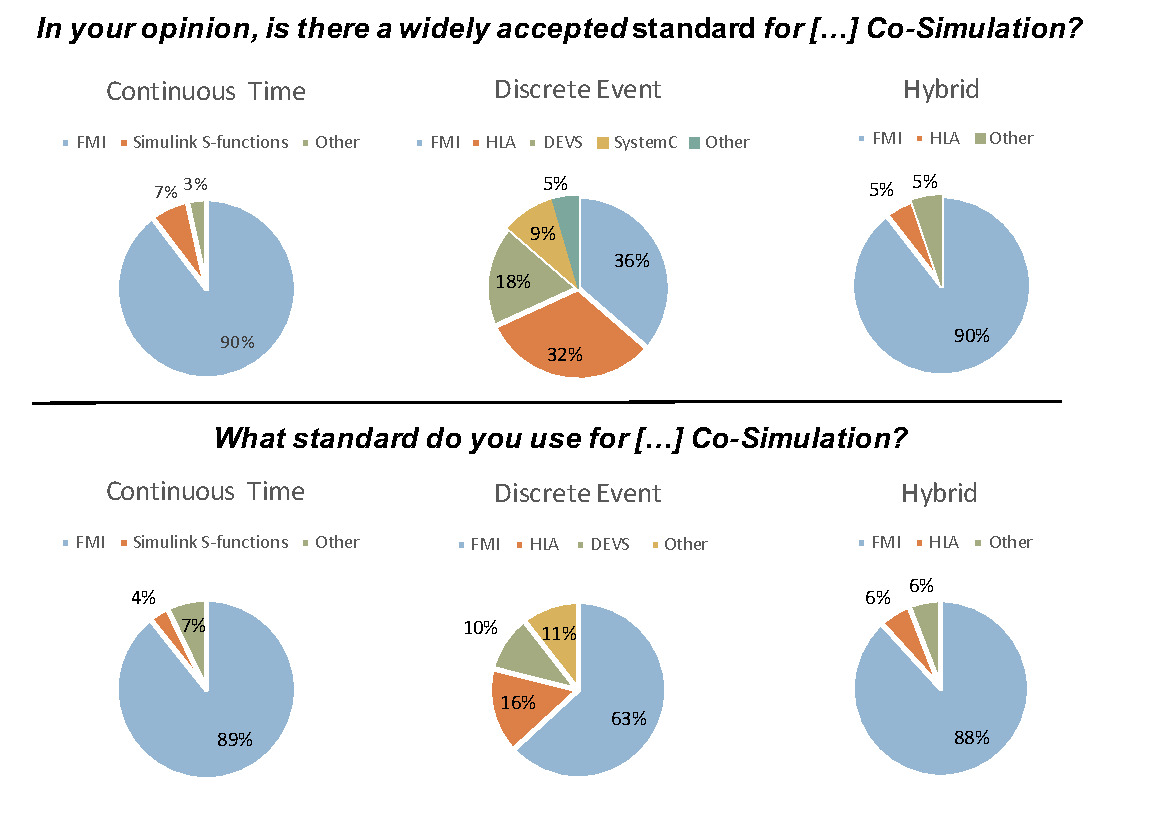
\includegraphics[width=1\textwidth]{Figures/Tools.pdf}
\caption{Widely accepted and used standards for co-Simulation. \claudio{I don't know if we mention this, but a threat to validity is the bias towards the FMI.}}
\label{fig:Standards}
\end{figure}

%\begin{figure}[h!]
%\centering
%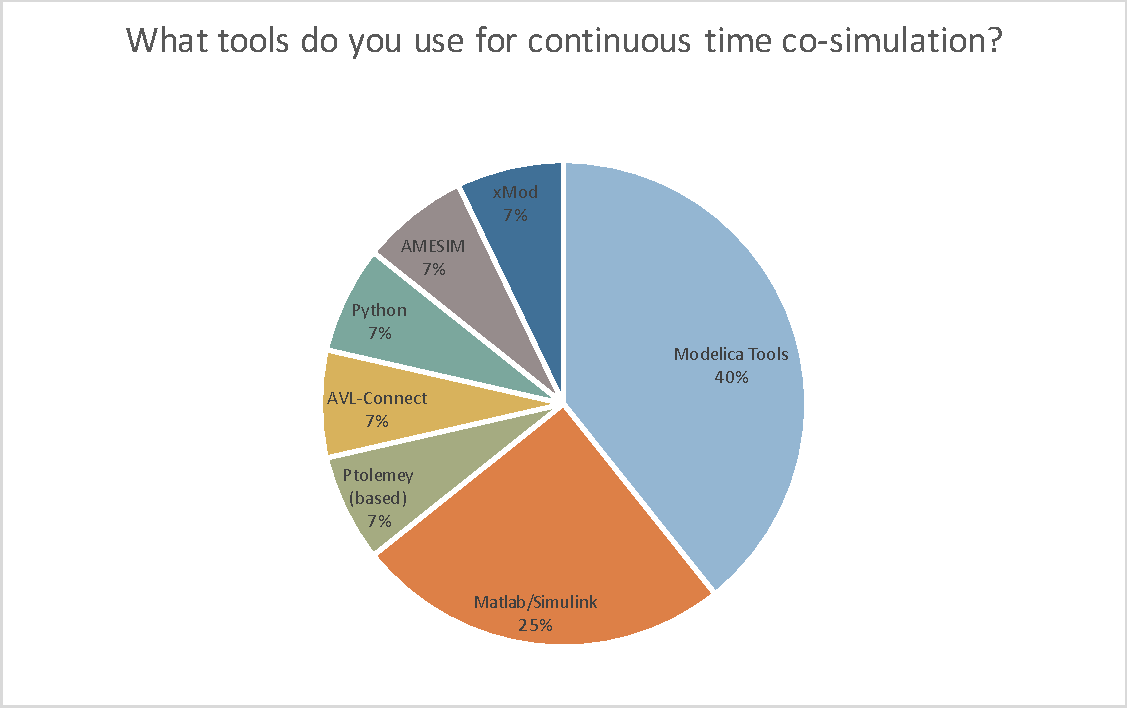
\includegraphics[width=1\textwidth]{Figures/Tools_coSim.pdf}
%\caption{Widely used tools for continuous time Co-Simulation}
%\label{fig:ToolsCont}
%\end{figure}

\claudio{We don't need the text below. It's redundant with the figure. Maybe just mention the preferred standard, and the least picked one.}
Experts in the field of co-simulation see FMI as a promising standard for continuous time, discrete event and hybrid co-simulation;  90 \% of the experts see FMI, 7 \% Simulink S-functions and 3 \% other standards as a widely accepted standard for continuous time co-simulation. 
For discrete event co-simulation  36 \% see FMI, 32 \% HLA, 18 \% DEVS formalism, 9 \% SystemC and 5 \% other standards as widely accepted. 
For hybrid so-simulation  90 \% see FMI, 5 \% HLA  and 5 \%  other standards as widely accepted. 
While for continuous time and hybrid co-simulation the responses for "widely accepted standards" and "standards which experts use" are similar, a different picture emerges for discrete event co-simulation. 
Only 36 \% of the experts state FMI as widely accepted for discrete event co-simulation; contrary to this, 63 \% of the experts use FMI for discrete event co-simulation. 
Details about research challenges and current barriers for FMI can be found in \cite{Schweiger2018b}.

In addition to promising standards, experts were asked what tools they use for co-simulation. The most common tools for continuous time co-simulation are Modelica tools and Matlab/Simulink. 
About half of the experts mentioned that they use (among other tools) \claudio{We don't need these parenthesis. It's obvious they will use other tools.} Modelica tools and about 40 \% of the experts mentioned that they use (among other tools) Matlab/Simulink. 
For discrete event co-simulation, no tool was significantly more frequently mentioned than others; very often, self-written tools were mentioned. 
Similarly, for hybrid co-simulation, no tool was significantly more frequently mentioned than others.

%\begin{figure}[h!]
%\centering
%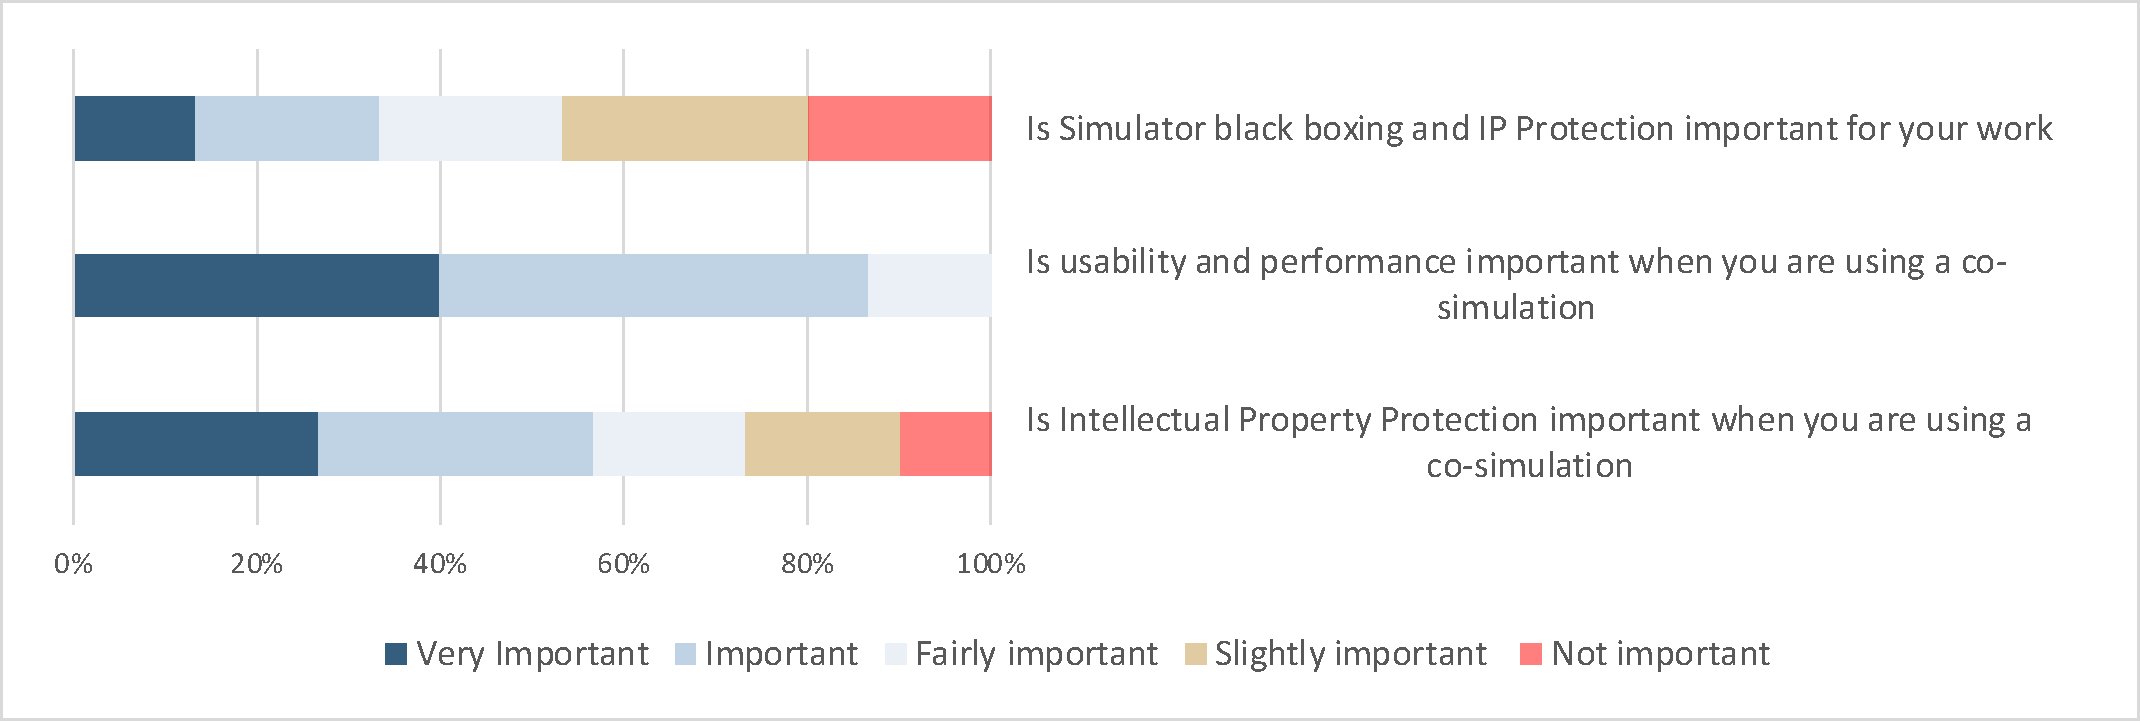
\includegraphics[width=1\textwidth]{Figures/Personal_1.pdf}
%\caption{xxxxx}
%\label{fig:xxxx}
%\end{figure}


\subsection{Current challenges}
In the first round of the Delphi study, experts commented on current challenges in co-simulation. 
Based on these responses and an extensive literature review, we formulated several statements regarding personal experiences. 
In the second round of the Delphi Study, experts were asked to rate those statements ("Have you experienced" [...]) based on a 6-point Likert scale from $1 = \text{``very frequently''}$ to $6 = \text{``never''}$. 
Table \ref{fig:challenges} summarizes the responses sorted according to how often experts experiences certain issues. 
A detailed discussion of the individual challenges goes beyond the scope of this survey; further information can be found in the references to the respective challenges in Table \ref{fig:challenges}.

\begin{table}[htbp]
\tiny
  \centering
  \caption{Experts assessments: Current challenges. Score: Very Frequently (6) Frequently (5) Occasionally (4) Rarely (3) Very Rarely (2) Never (1). \claudio{Maybe in the method section, we should explain what the interpolated median is, and how it should be interpreted. Remember that our readers are not experts in empirical studies.}}
    \begin{tabularx}{1\linewidth}{
        X
        >{\color{black}}R{0.8cm}
        >{\color{black}}R{0.8cm}
        >{\color{red}}R{0.8cm}
        <{\color{black}}
    }
    %\toprule    
    & \thead{Mean} & \thead{Median} & \thead{Interp.\\Median} \\
    \midrule
        Difficulties in practical aspects, like IT-prerequisites in cross-company collaboration  & 4.7   & 5.0   & 4.7 \\
            Difficulties due to insufficient communication between theorists and practitioners   & 4.4   & 5.0   & 4.6 \\
    Difficulties in judging the validity of a co-simulation   & 4.6   & 4.0   & 4.4 \\
    Difficulties in how to define the macro step size for a specific co-simulation \cite{Benedikt2013b,Busch2011,Gomes2017}  & 4.3   & 4.0   & 4.3 \\
        Numerical stability issues of co-simulation \cite{Busch2016,Gomes2017,Arnold2010}  & 4.4   & 4.0   & 4.3 \\
    Issues with algebraic loops \cite{Kubler2000,Gomes2017} & 4.2   & 4.0   & 4.2 \\

    Difficulties in how to define tolerances  & 4.3   & 4.0   & 4.0 \\
    Issues because of too simplistic extrapolation functions  & 3.5   & 4.0   & 3.6 \\
    Difficulties in choosing the right co-simulation orchestration algorithm (master)  & 3.6   & 3.0   & 3.4 \\
    \bottomrule
    \end{tabularx}%
   
  \label{tab:LS}%
\end{table}%

Experts frequently have \textit{"Difficulties in practical aspects, like IT-prerequisites in cross-company collaboration"} ($M=5.0; IM = 4.7$) and \textit{"Difficulties due to insufficient communication between theorists and practitioners"} ($M=5.0; IM = 4.6$). 
With the exception of \textit{"Issues because of too simplistic extrapolation functions"} and \textit{"Difficulties in choosing the right co-simulation orchestration algorithm (master)"}, all challenges are assessed by the experts with a interpolated median value greater or equal to 4 which corresponds to the answer "Occasionally"; this fact confirms that the challenges we provided are indeed challenges faced by the experts. 


\subsection{Research needs}
Based on responses in the first round of the Delphi study and an extensive literature review, experts where asked about research topics in the field of co-simulation that have not received enough attention up to now.
Table \ref{fig:ResearchNeeds} summarizes the responses which are sorted in ascending order of topics that have not received enough attention up to now. 
Based on the evaluation of the experts for each question, we have classified each topic according to whether there is a need for research: topics with an Intermediate Median score of $5.5$ or higher require ``Intensive Research Activity''.
Topics with an Interpolated Median between $5.5$ and $5.0$ require `` Moderate Research Activity'' and topics with an Interpolated Median score less than $5.0$ require `` Limited to No Research Activity''.

\gerald{link to literature (the category "Intensive Research Activity"}

\begin{table}[htbp]
\tiny
  \centering
  \caption{Experts assessments: Research needs. Score: Entirely agree (7) Mostly agree (6) Somewhat agree (5) Neither agree nor disagree (4) Somewhat disagree (3) Mostly disagree (2) Entirely disagree (1).}
    \begin{tabularx}{1\linewidth}{
        X
        >{\color{black}}R{0.8cm}
        >{\color{black}}R{0.8cm}
        >{\color{red}}R{0.8cm}
        <{\color{black}}
    }
    %\toprule    
    & \thead{Mean} & \thead{Median} & \thead{Interp.\\Median} \\
    \midrule
    Theoretical understanding of how to accurately include different kinds of controllers in different co-simulation approaches  & 5.5   & 6.0   & 5.9 \\
    Representation and enforcement of model validity assumptions  & 5.6   & 6.0   & 5.8 \\
    Hybrid co-simulation (e.g., variable structure systems, switched systems, impulsive systems, etc...)  & 5.8   & 6.0   & 5.8 \\
    Impact of coupled error controlled algorithms & 5.7   & 6.0   & 5.8 \\
    Uncertainty quantification/propagation & 5.6   & 6.0   & 5.8 \\
    Impact of updating inputs (and the discontinuity it introduces) in the subsystems  & 5.6   & 6.0   & 5.7 \\
    Acausal approaches for co-simulation  & 5.6   & 6.0   & 5.7 \\
    Impact of using different tolerances in a sub-component on the overall simulation  & 5.3   & 6.0   & 5.5 \\
    Numerical stability & 5.3   & 5.0   & 5.4 \\
    Systematic categorization of different co-simulation approaches, including a better understanding of how their model of computations and requirements overlap and differ & 5.2   & 5.0   & 5.4 \\
    Usability and performance  & 4.9   & 5.0   & 5.1 \\
    Simultaneous events  & 5.7   & 6.0   & 5.8 \\
    Integration of a wide variety of simulators despite different structures (while achieving/maintaining high performance)  & 4.8   & 5.0   & 4.9 \\
    Parallelization  & 4.6   & 5.0   & 4.9 \\
    Simulator black boxing and IP Protection & 4.1   & 4.0   & 4.1 \\


    \bottomrule
    \end{tabularx}%
   
  \label{tab:Research}%
\end{table}%

To (i) evaluate controversial assessments regarding research needs from the first Delphi round and from literature as well as to (ii) provide a different perspective on research needs, additional questions to the questions in \ref{tab:Research} were defined. 
Experts where asked if several statements are important for their work. The average score of each Likert-scale question (Very important=5 to Not important=1) was calculated. 
The statements $S_1$ \textit{"Is usability and performance important when you are using a co-simulation"} ($Mean = 4.3, M = 4.0, IM = 4.3)$) and $S_2$: \textit{"Is Intellectual Property Protection important when you are using a co-simulation"} ($Mean = 3.9, M = 4.0, IM = 3.7)$) were assessed as important.
Compared to the previous, \textit{"Is Simulator black boxing and IP Protection important for your work"} was assessed as not so important ($Mean = 3.5, M = 3.0, IM = 2.7)$).

\gerald{An expert mentioned: This connects to the fundamental idea of what is the idea (or goal) with hybrid co-simulation? Is the intention to allow, with hybrid co-simulation, the same flexibility as there is in a monolithic simulation (with everything that this entails)? To me co-simulation should be about coupling of "large" subsystems - not for instance being able to connect a circuit with resistors as separate subsystems. I image that the two different views will have very different requirements on a hybrid co-simulation. My view is also that most of this is largely unexplored and needs more research regarding the numerical properties with such a scheme."}

\gerald{"An expert mentioned that from a theoretical side the subject is quite well covered. What is missing are implementations, especially for popular tools."}

\gerald{An expert mentioned: I also have the impression, that there is only limited awareness about the problems that can arise in hybrid co-simulation. Most users don't understand whether problems arise due to shortcomings of standards, tool implementation or usage. I already referenced this before, but this paper gives a simple example: FMI-based co-simulation of hybrid closed-loop control system models}


Furthermore, experts where asked to which extent they agree on several statements. Seven-point Likert scale have been used to measure responses (Entirely agree =7 to Entirely disagree = 1). 

Experts mostly agree to the statement \textit{"For academia it is difficult to experiment with different co-simulation approaches as there is a huge learning curve: in terms of learning the specification and also gaining access to models as well as being able to make changes to existing approaches and test new ideas"} ($Mean = 5.5, M = 6.0, IM = 5.8)$) and somewhat agree to the statements \textit{"A clearer categorization of different co-simulation approaches would help for your particular field of work"} ($Mean = 5.8, M = 5.0, IM = 5.1)$) and \textit{"The major benefit of co-simulation is to increase performance, when compared to a monolithic simulation"} ($Mean = 4.7, M = 5.0, IM = 4.7)$); they neither agree nor disagree to the statement \textit{"A acausal approaches can boost the use of co-simulation in your field"} ($Mean = 5.1, M = 4.0, IM = 4.3)$).

\claudio{Now I realize that the question "Is usability and performance important when you are using a co-simulation" is a terrible question... because we cannot be sure whether it refers to performance or usability! xD. However, note that in research needs, there are some people disagreeing with the need for more research in that. Maybe because usability has not been posed as a scientific problem?}
\gerald{Dammmit - I agree...any ideas? @Sepp? I would suggest to leave it as it is}

%\claudio{Also, the example provided in the  "difficulties in judging the validity of a co-simulation, i.e. estimating the associated
%communication error" question is not a validity problem. A validity problem is related to %whether the model captures the essence of the physical system. It has nothing to do with co-simulation.
%Also, we should capitalize the questions, to make them nicer...}
\claudio{It's interesting that simulator black boxing and IP protection are pointed out as having received enough attention lately.}

\subsection{SWOT-AHP}
The results of the SWOT-AHP analysis are presented in Table \ref{table1} and in Fig. \ref{fig:SWOT}. The factors for each group are on the lines in the four sectors. The lengths of the lines indicate the group priority, respectively the relative overall importance of the four SWOT-groups. The three circles per group indicate the global factor priorities; the longer the distance between the respective group/factor and the origin, the higher the overall importance of this group/factor.

\begin{table}[]
\caption{Result SWOT-AHP}
\label{table1}
\resizebox{\textwidth}{!}{%
\begin{tabular}{llllll}
\hline
\multicolumn{2}{l}{\textbf{SWOT Factors}} & \textbf{CR} & \textbf{\begin{tabular}[c]{@{}l@{}}group\\ priority\end{tabular}} & \textbf{\begin{tabular}[c]{@{}l@{}}local \\ priority\\ (rank)\end{tabular}} & \textbf{\begin{tabular}[c]{@{}l@{}}global\\ priority\\ (rank)\end{tabular}} \\ \hline
\multicolumn{2}{l}{\textbf{Strenghts (internal)}} & 0.085 & 0.34 &  &  \\
\multicolumn{2}{l}{\textit{Sa: It supports cross-discipline developments}} &  &  & 0.35 (2) & 0.117 (3) \\
\multicolumn{2}{l}{Sb: It supports cross-company cooperations} &  &  & 0.21 (3) & 0.072 (7) \\
\multicolumn{2}{l}{\textit{\begin{tabular}[c]{@{}l@{}}Sc: Every sub-system can be implemented in a tool that meets the particular\\ requirements for the domain, the structure of the model and the simulation algorithm\end{tabular}}} &  &  & 0.44 (1) & 0.148 (2) \\ \hline
\multicolumn{2}{l}{\textbf{Weaknesses (internal)}} & 0.013 & 0.16 &  &  \\ \hline
\multicolumn{2}{l}{\textit{Wa: Computational performance of co-simulation compared to monolythic simulation}} &  &  & 0.34 (2) & 0.056 (9) \\
\multicolumn{2}{l}{\textit{Wb: Robustness of co-simulation compared to monolythic simulation}} &  &  & 0.41 (1) & 0.067 (8) \\
\multicolumn{2}{l}{\textit{Wc: Licenses for all programs are required to couple different simulation programs}} &  &  & 0.24 (3) & 0.039 (12) \\ \hline
\multicolumn{2}{l}{\textbf{Opportunities (external)}} & 0.003 & 0.33 &  &  \\ \hline
\multicolumn{2}{l}{\textit{Oa: Growing co-simulation community/growing industrial adoptaion}} &  &  & 0.29 (2) & 0.094 (4) \\
\multicolumn{2}{l}{\textit{\begin{tabular}[c]{@{}l@{}}Ob: User-friendly tools (pre-defined master algorithms, integrated error estimation,\\ sophisticated analysis to determine best parametrization of solvers and master algorithms)\end{tabular}}} &  &  & 0.47 (1) & 0.153 (1) \\
\multicolumn{2}{l}{\textit{\begin{tabular}[c]{@{}l@{}}Oc: Better communication between theoretical/numerical part, implementation and\\ application/industry\end{tabular}}} &  &  & 0.25 (3) & 0.080 (6) \\ \hline
\multicolumn{2}{l}{\textbf{Threats (external)}} & 0.003 & 0.18 &  &  \\ \hline
\multicolumn{2}{l}{\textit{Ta: Insufficient knowledge/information of user in co-simulation may lead to improper use}} &  &  & 0.28 (3) & 0.088 (5) \\
\multicolumn{2}{l}{\textit{Tb: Incompatibility of different standards and co-simulation approaches}} &  &  & 0.41 (1) & 0.043 (11) \\
\multicolumn{2}{l}{\textit{\begin{tabular}[c]{@{}l@{}}Tc: Lack of exchange/cooperation between theoretical/numerical part, implementation and\\ application/industry.\end{tabular}}} &  &  & 0.31 (2) & 0.044 (10) \\ \hline
\end{tabular}%
}
\end{table}

\begin{figure}[h!]
\centering
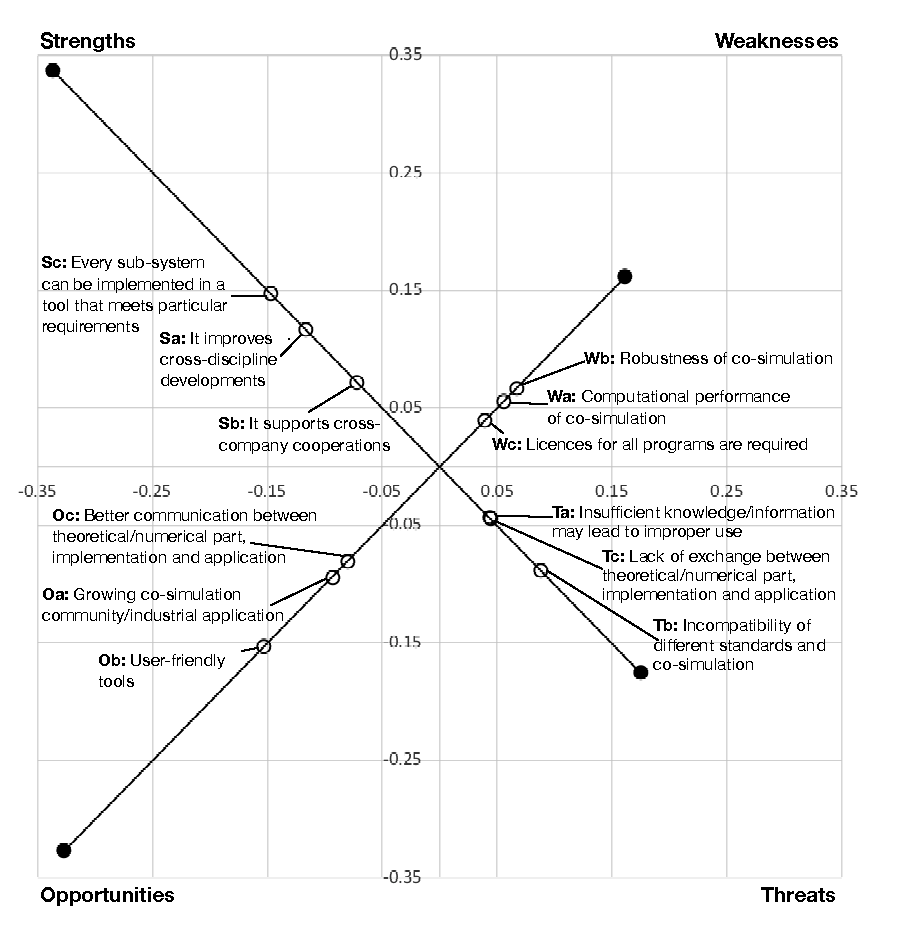
\includegraphics[width=1\textwidth]{Figures/SWOTAHPcosim.eps}
\caption{Research needs}
\label{fig:SWOT}
\end{figure}


The results of the SWOT-AHP analysis indicate that strengths and opportunities factors predominate. The four factors with the highest global priorities are within the Strengths and Opportunities group. The factor with the highest global priority is the external opportunity of User-friendly tools including pre-defined master algorithms, integrated error estimation, etc. The factor with the second highest global priority is the internal strengths that sub-systems can be implemented in a tool that meets the particular requirements for the domain, the structure of the model and the simulation algorithm. The factor with the third highest global priority is the internal strengths that co-simulation supports cross-discipline developments. Some experts mentioned further SWOT factors. As a strengths, some experts mentioned that parallel modeling and simulation can reduce the overall modeling and simulation time. Another strength is that co-simulation approaches supports modularity and the reuse of components. An expert stated the lack of sufficiently strong theory as a weakness of co-simulation. In the group opportunities, an expert mentioned the integration of tools for the application of formal methods. On expert pointed out that a threat could be that some big companies may be actively against the widespread use of co-simulation.

An interesting outcome is that the groups of Strengths and Opportunities are seen much more important than Weaknesses and threats. This follows due to the priority of the first two groups, which are approximately twice as high as the latter two. The consistencies of the pairwise comparisons was checked. All consistency ratios are below xxx. It can be concluded, that the results are consistent. 

\claudio{It's strange that so many people use FMI for discrete event co-simulation... and at the same time the FMI committee is trying to improve the standard to support DE based co-simulation! 
As a result, a critic we might get in our study is that there is no balance in the selection of experts.
We must defend from this criticism in the discussion section.}



%\claudioi{Also, overall we should summarize the results as we introduce each figure/table. So that the reader can opt for just read the text (ignore the figs) and still get a sense of what the main results are.}

%\claudioi{To follow good practice, every figure/table must be within a float environment. If we need to keep figures within a specific section, then we should use the appropriate positioning parameters (and the float package).}


\section{Conclusion}

The present paper presents an expert assessment on co-simulation, taking on the social and empirical aspect, with a focus on promising standards and tools, current challenges and research needs. 
As a methodological foundation of this study, the Delphi method was adopted.
Furthermore, a quantitative analysis of the SWOT of co-simulation utilizing the Analytic Hierarchy Process has been conducted.
The authors consider the following findings from the empirical data as the most important:

\begin{compactitem}
\item Experts consider FMI as the most promising standards for continuous time, discrete event  and  hybrid  co-simulation;
\item Experts frequently have difficulties in practical aspects, like IT-prerequisites in cross-company collaboration and difficulties due to
insufficient communication between theorists and practitioners;
\item Research needs xxxxxx; and 
\item The  results  of  the  SWOT-AHP  analysis  indicate that strengths and opportunities factors predominate.  The factor with the  highest  score  is  the  external  opportunity  of  User-friendly  tools  including pre-defined master algorithms, integrated error estimation, etc.;
\end{compactitem} \leavevmode
\\
It is our hope that the results of this study increase transparency and facilitate a structured development of co-simulation standards and tools.








\section*{Acknowledgement}
We want to thank all experts who participated in the study. 
\section{References}

\bibliography{Literature,Mendeley,mendeley_v2,bib_claudio}

\section{Appendix}

\claudio{Since this is a journal paper, I suggest that we get rid of the appendix: we move these figures to the journal body.}

\begin{figure}[h!]
\centering
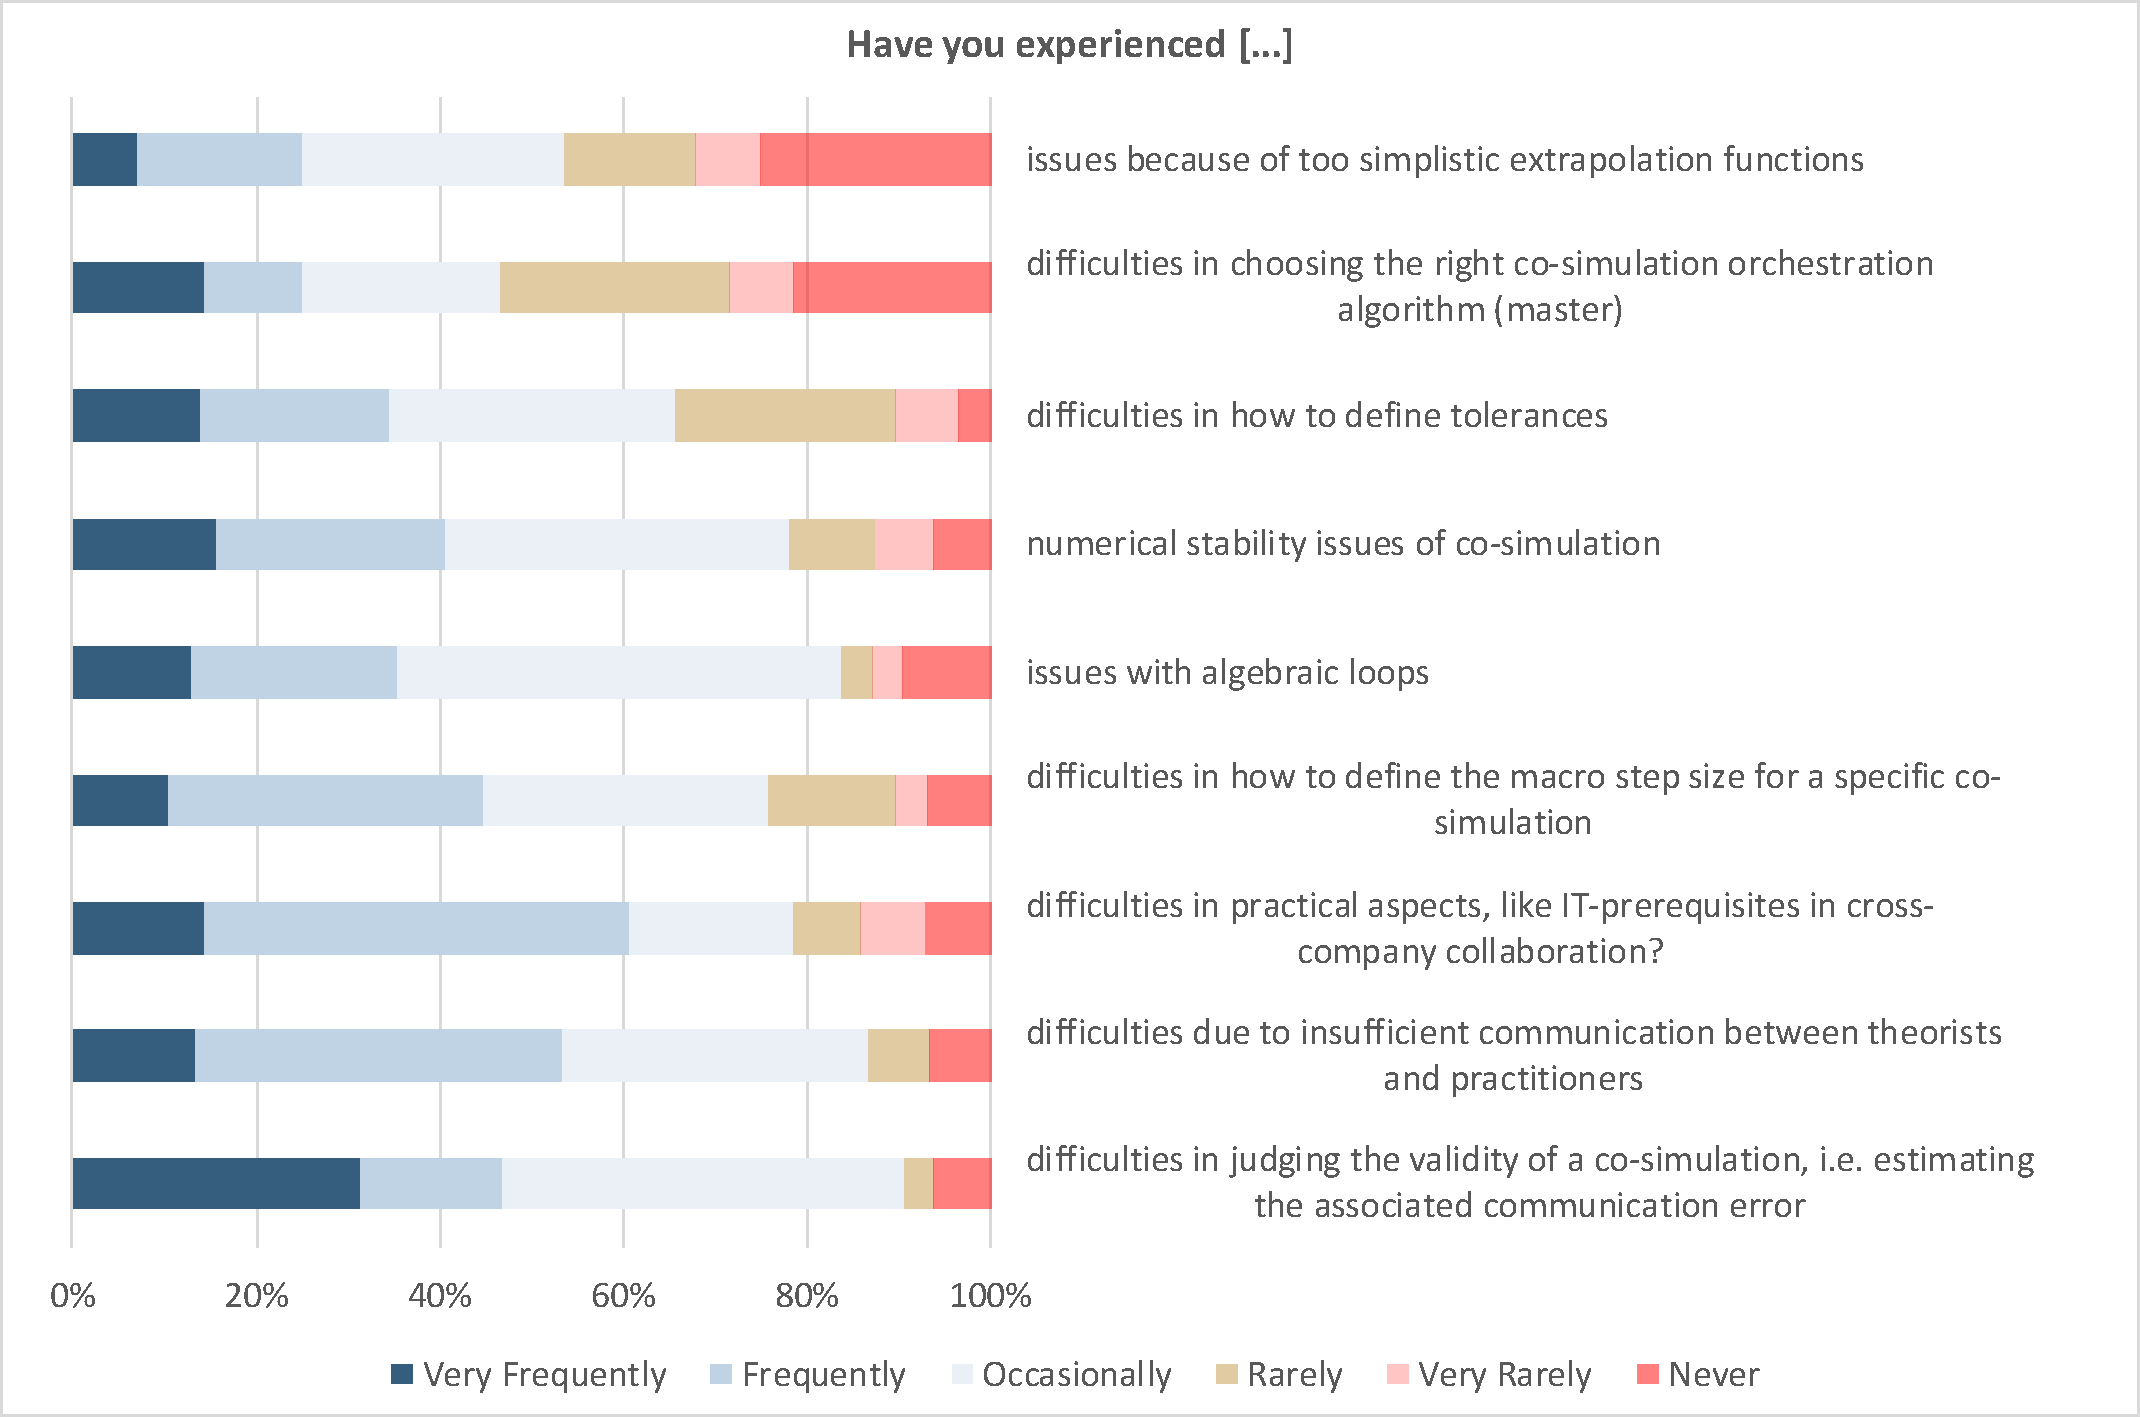
\includegraphics[width=1\textwidth]{Figures/Personal.pdf}
\caption{Current challenges}
\label{fig:challenges}
\end{figure}


\begin{figure}[h!]
\centering
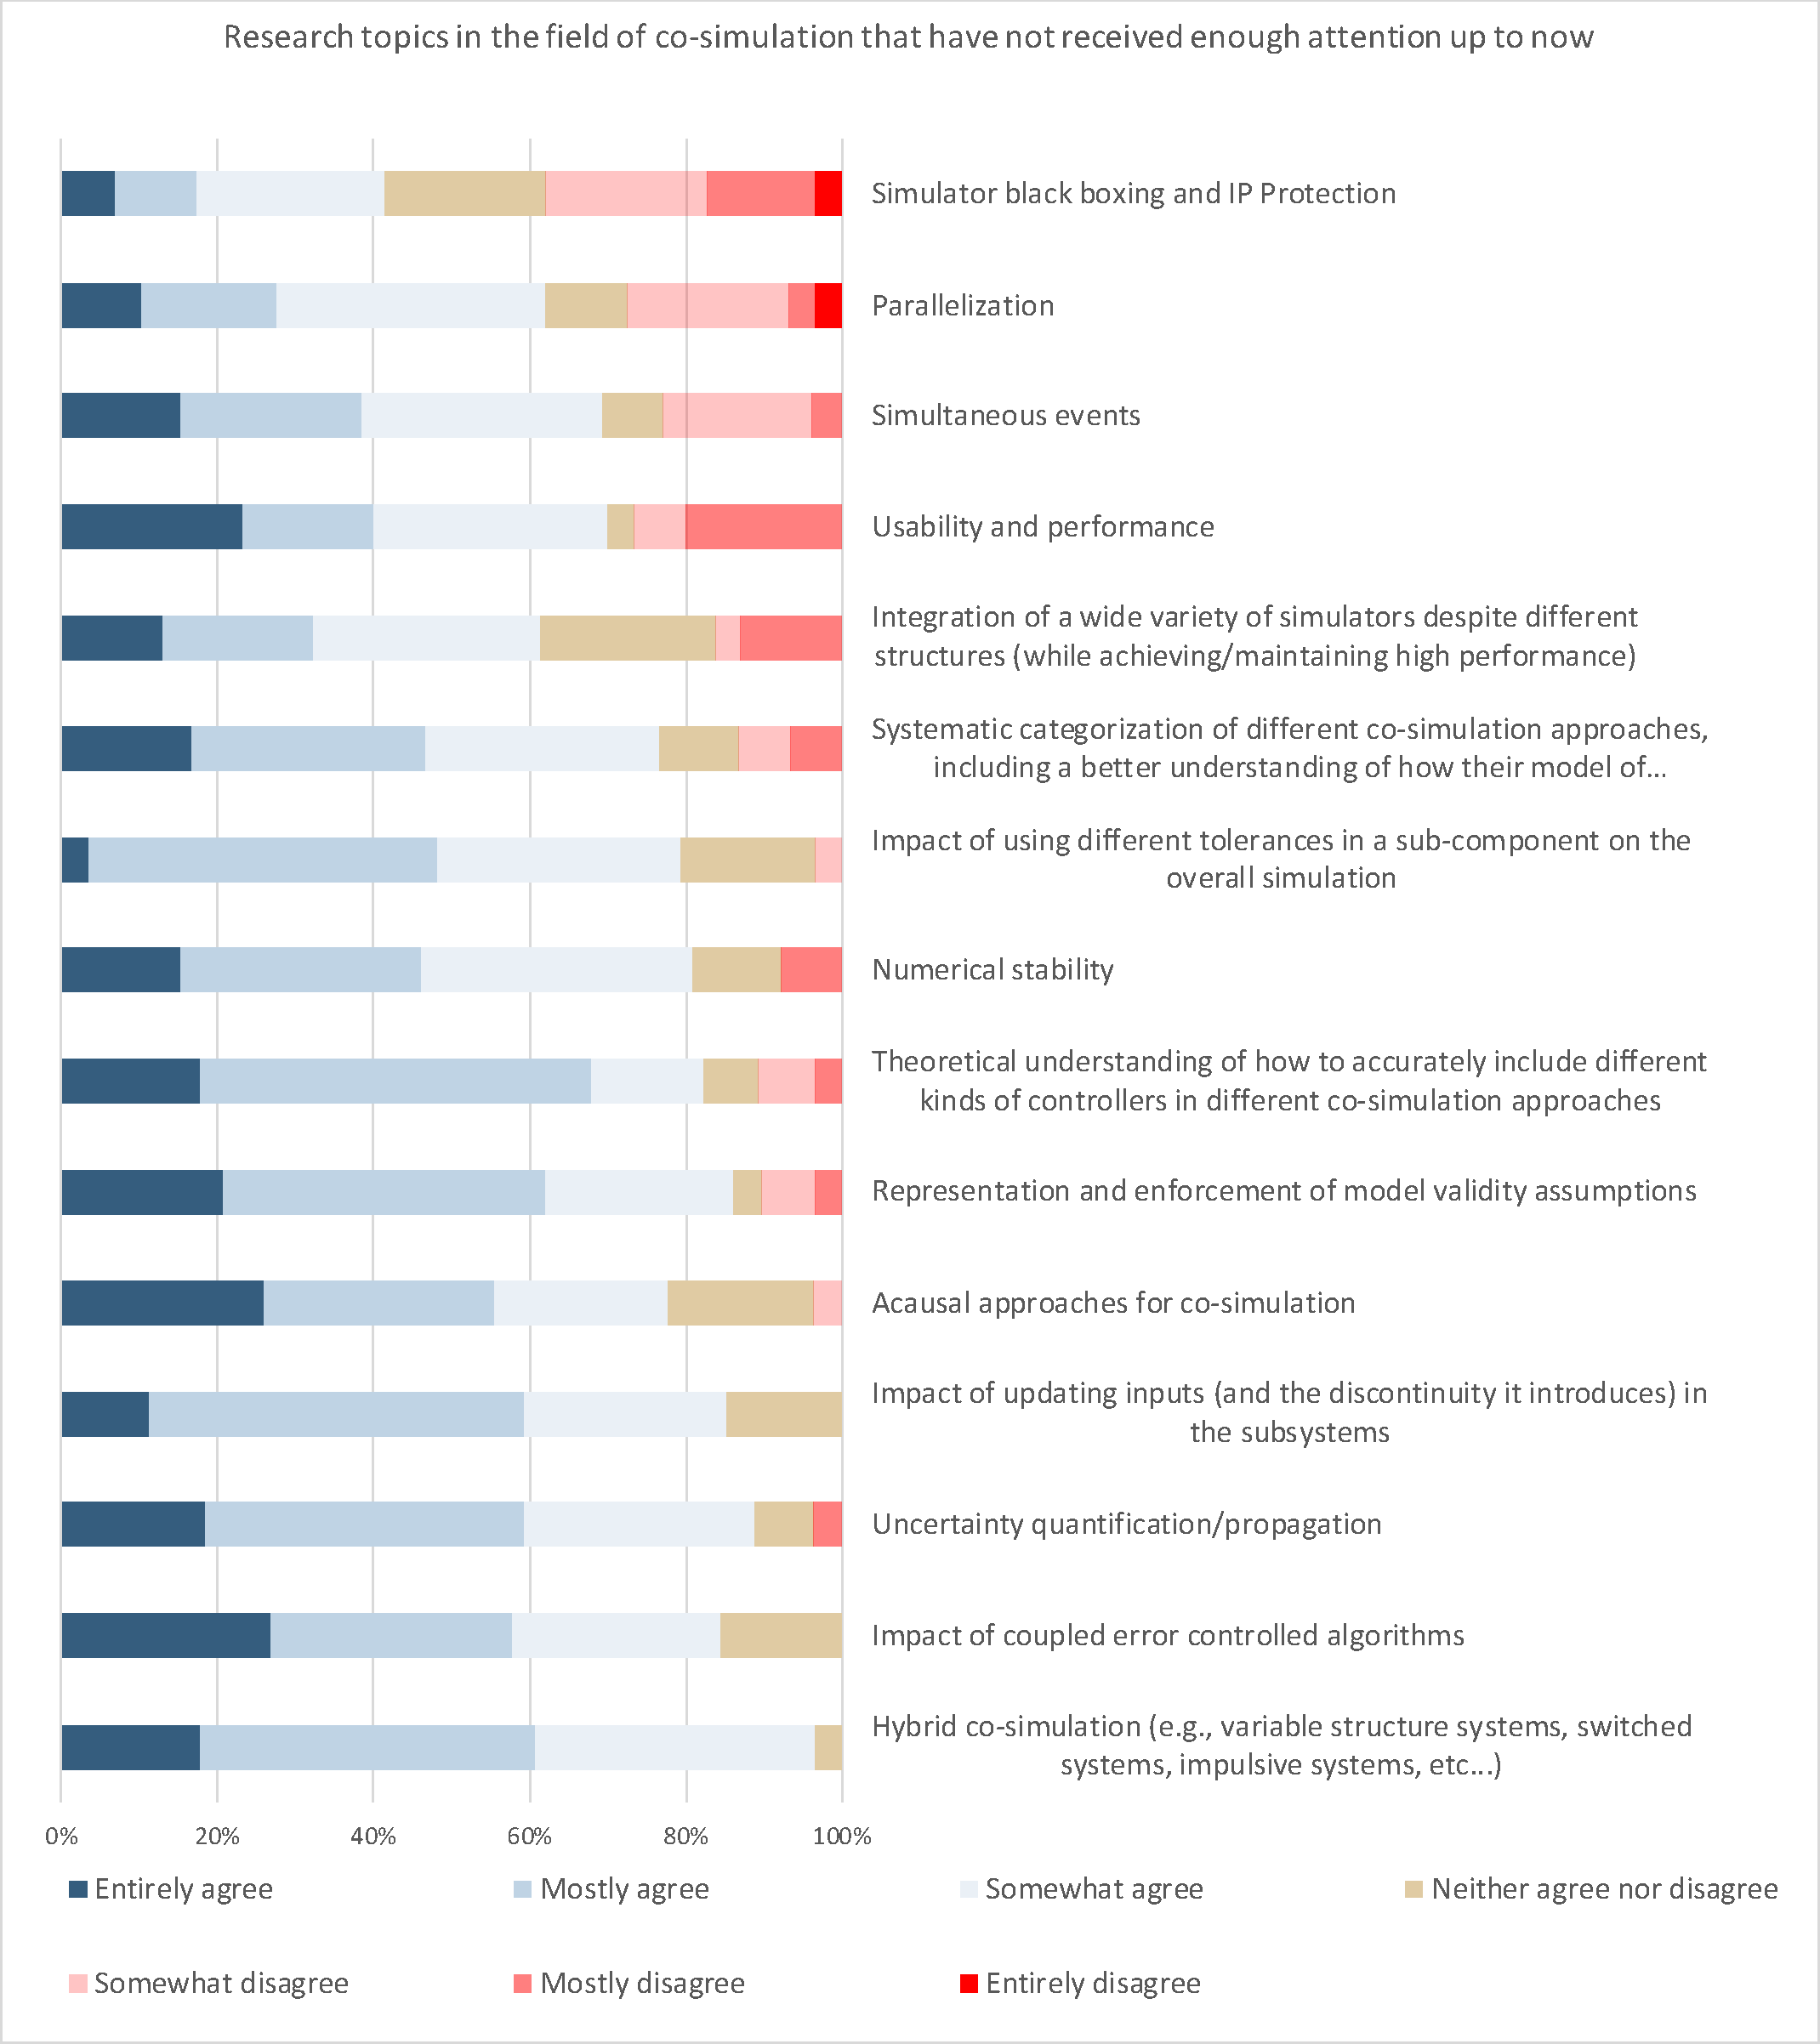
\includegraphics[width=1\textwidth]{Figures/Research.pdf}
\caption{Research needs}
\label{fig:ResearchNeeds}
\end{figure}

\newpage
\end{document}
